\chapter{Dynamiek van het cytoskelet en celbeweging}\label{ch:b3:cytoskeleton-motility}

Een neutrofiel die een bacterie door een weefsel achtervolgt kruipt
tien micrometer per minuut en verandert binnen seconden van richting
wanneer het spoor verschuift. Een blaasje met neurotransmitter dat in
het cellichaam van een motorisch neuron is gemaakt legt een meter door
het axon naar de voet af, gesleept door een motoreiwit dat stappen van
acht nanometer zet, honderd per seconde, veertien dagen lang. De
trilharen die de luchtpijp bekleden slaan twaalf keer per seconde in
gecoördineerde golven die het stof van een dag naar de keel voeren. Dit
alles wordt gedaan door drie soorten eiwitfilament die zich in seconden
samenstellen en weer uiteenvallen, en door motoren die per stap één
molecuul ATP verbranden. Het cytoskelet is helemaal geen skelet in de
zin van een vast geraamte; het is een verzameling polymeren in
voortdurende omzet, waarvan de dynamiek het mechanisme van vorm,
deling en beweging \emph{is}. Dit hoofdstuk behandelt de polymeren en
hun kinetiek, de motoren en de natuurkunde die hen begrenst, het
kruipen van een cel, en het slaan van trilharen en zweepstaarten.

\section{Drie polymeren}

\begin{definition}[Actinefilamenten, microtubuli, intermediaire filamenten]\label{def:b3:cytoskeleton-motility:filaments}
\index{actinefilament}\index{microtubulus}\index{intermediair filament}\index{polariteit!van filamenten}\index{centrosoom}
Een \emph{actinefilament} is een tweestrengs helicaal polymeer van
bolvormig actine, \qty{7}{nm} dik, met elke subeenheid \qty{2.7}{nm}
langs de as, en het is polair: het \emph{gekartelde} (plus)uiteinde
groeit sneller dan het \emph{gepunte} (min)uiteinde, en elke
subeenheid draagt een ATP dat na de inbouw wordt gehydrolyseerd. Een
\emph{microtubulus} is een holle buis met een buitendiameter van
\qty{25}{nm}, opgebouwd uit dertien protofilamenten van
$\alpha\beta$-tubulinedimeren (\qty{8}{nm} per dimeer), eveneens
polair, met een \emph{plusuiteinde} dat sneller groeit en een
\emph{minuiteinde} dat meestal is verankerd aan het \emph{centrosoom}
bij de kern; de $\beta$-subeenheid hydrolyseert haar GTP na de inbouw.
Een \emph{intermediair filament} is een touw van \qty{10}{nm} van
coiled-coil-eiwitten (keratines in epitheel, vimentine in mesenchym,
neurofilamenten in axonen, lamines onder het kernmembraan), apolair,
zonder nucleotide en veel stabieler --- eerder een kabel die trek
opvangt dan een dynamische baan. Actine zit vooral onder het
plasmamembraan en in uitstulpingen; microtubuli stralen uit het
centrosoom en dienen als de banen van transport over lange afstand en
als spoelfiguur; intermediaire filamenten geven een cel en haar kern
hun mechanische veerkracht.
\end{definition}

\begin{omfigure}
\begin{tikzpicture}[every node/.style={font=\scriptsize}, >=stealth]
  % actin
  \begin{scope}
    \foreach \i in {0,...,11} { \fill[omThm!70] ({\i*0.4},{0.12*sin(\i*60)}) circle (0.17); }
    \node[below, align=center] at (2.2,-0.5) {actinefilament, \qty{7}{nm}\\tweestrengs helix, ATP-actine\\subeenheid \qty{2.7}{nm} langs de as};
    \node[left] at (-0.3,0) {$-$ gepunt}; \node[right] at (4.6,0) {gekarteld $+$};
  \end{scope}
  % microtubule
  \begin{scope}[xshift=7.2cm]
    \draw[thick, fill=omDef!25] (0,-0.55) rectangle (4.4,0.55);
    \foreach \y in {-0.35,-0.15,0.05,0.25} \draw[omDef] (0,\y) -- (4.4,\y);
    \foreach \x in {0.4,0.8,...,4.0} \draw[omDef] (\x,-0.55) -- (\x,0.55);
    \draw[thick] (4.4,0) ellipse (0.18 and 0.55); \draw[thick, fill=white] (4.4,0) ellipse (0.09 and 0.38);
    \node[below, align=center] at (2.2,-0.65) {microtubulus, \qty{25}{nm}\\13 protofilamenten van $\alpha\beta$-tubuline (GTP)\\dimeer \qty{8}{nm} lang};
    \node[left] at (-0.2,0) {$-$}; \node[right] at (4.7,0) {$+$};
  \end{scope}
  % intermediate filament
  \begin{scope}[yshift=-2.9cm, xshift=3.6cm]
    \foreach \dd in {-0.12,0,0.12} \draw[omMeth!70!black, thick] plot[domain=0:4.4, samples=60] (\x, {\dd + 0.1*sin(\x*200 + \dd*400)});
    \node[below, align=center] at (2.2,-0.4) {intermediair filament, \qty{10}{nm}\\coiled-coil-touw (keratine, vimentine, lamine), geen polariteit, geen nucleotide};
  \end{scope}
\end{tikzpicture}

{\small De drie filamenten, op schaal naar diameter. De polymeren van
actine en tubuline zijn polair en hydrolyseren na het samenstellen een
nucleotide, en dat maakt hen dynamisch; het intermediaire filament is
een apolair touw dat voor uithoudingsvermogen is gebouwd.}
\end{omfigure}

\begin{omfigure}
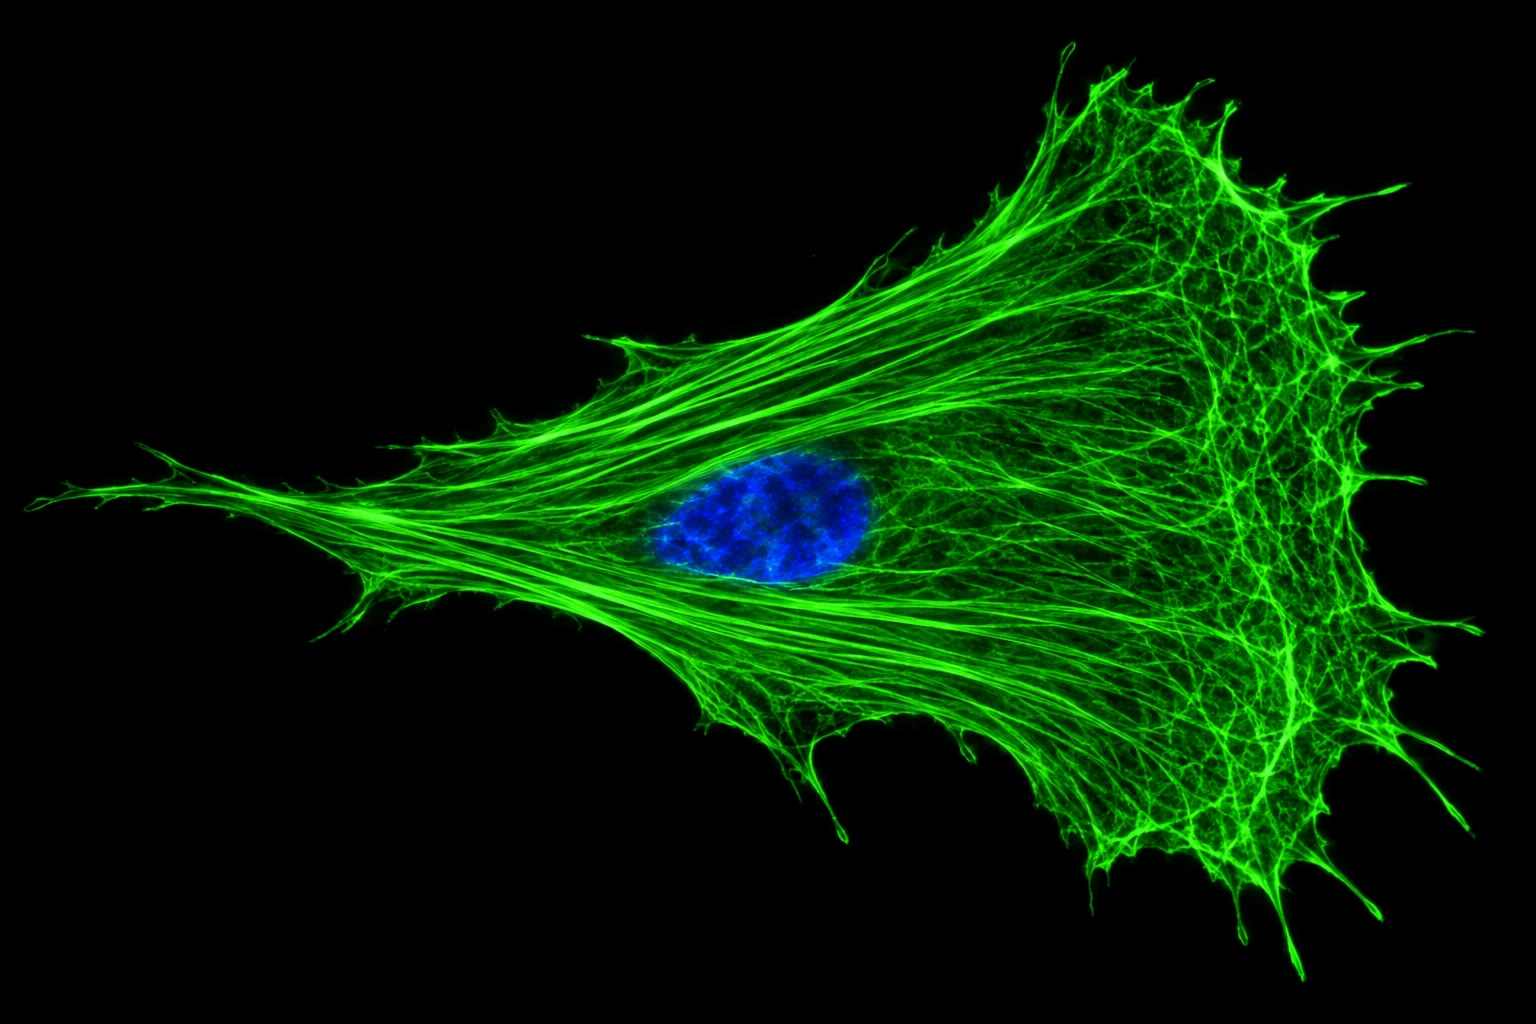
\includegraphics[width=0.54\linewidth]{images/book5/ai/b5-09-fibroblast-actin.jpg}\hspace{0.03\linewidth}
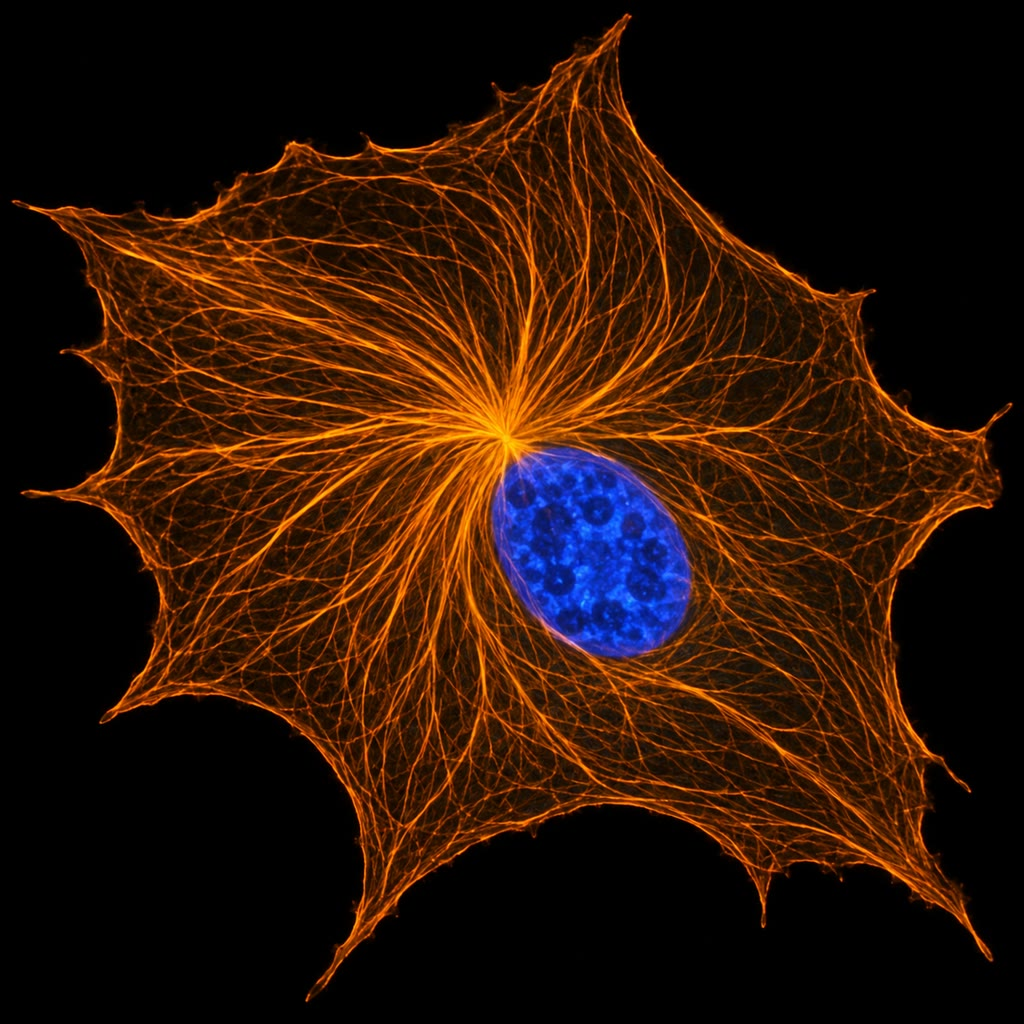
\includegraphics[width=0.36\linewidth]{images/book5/ai/b5-09-microtubules.jpg}

{\small Links: actine (groen) in een migrerende fibroblast ---
spanningsvezels door het cellichaam, een dicht netwerk aan de brede
voorrand rechts. Rechts: \omterm{def:b3:cytoskeleton-motility:filaments}{microtubuli} (oranje) die vanaf het \omterm{def:b3:cytoskeleton-motility:filaments}{centrosoom}
naast de kern (blauw) naar de celrand uitstralen.}
\end{omfigure}

\section{De kinetiek van een polymeer}

\begin{theorem}[Kritische concentratie en treadmilling]\label{thm:b3:cytoskeleton-motility:treadmilling}
\index{kritische concentratie}\index{treadmilling}
Laat een uiteinde van een filament subeenheden toevoegen met snelheid
$k_{\text{on}}C$, waarin $C$ de concentratie vrij monomeer is, en ze
verliezen met snelheid $k_{\text{off}}$. Het uiteinde groeit wanneer
$C$ boven zijn \emph{\omterm{thm:b3:cytoskeleton-motility:treadmilling}{kritische concentratie}}
$C_{c} = k_{\text{off}}/k_{\text{on}}$ ligt en krimpt eronder. Hebben
de twee uiteinden verschillende \omterm{thm:b3:cytoskeleton-motility:treadmilling}{kritische concentraties}, $C_{c}^{+}
< C_{c}^{-}$, dan is in de evenwichtstoestand waarin het filament noch
langer noch korter wordt de monomeerconcentratie
\[
C_{\text{ss}} = \frac{k_{\text{off}}^{+} + k_{\text{off}}^{-}}
{k_{\text{on}}^{+} + k_{\text{on}}^{-}},
\qquad C_{c}^{+} < C_{\text{ss}} < C_{c}^{-},
\]
en groeit het plusuiteinde terwijl het minuiteinde met dezelfde
snelheid krimpt,
$J = k_{\text{on}}^{+}C_{\text{ss}} - k_{\text{off}}^{+} > 0$:
subeenheden stromen van plus naar min door het filament ---
\emph{treadmilling} --- ten koste van één gehydrolyseerd nucleotide per
subeenheid.
\end{theorem}
\begin{proof}
De nettosnelheid aan een uiteinde is $k_{\text{on}}C - k_{\text{off}}$,
nul bij $C_{c}$. Een constante lengte vergt dat de som van de twee
nettosnelheden verdwijnt, wat $C_{\text{ss}}$ geeft; die ligt tussen de
twee \omterm{thm:b3:cytoskeleton-motility:treadmilling}{kritische concentraties} omdat zij er een gewogen gemiddelde van is
($C_{\text{ss}} =
(k_{\text{on}}^{+}C_{c}^{+} + k_{\text{on}}^{-}C_{c}^{-})/(k_{\text{on}}^{+}
+ k_{\text{on}}^{-})$). Boven $C_{c}^{+}$ groeit het plusuiteinde;
onder $C_{c}^{-}$ krimpt het minuiteinde; de stroom is de nettosnelheid
van het plusuiteinde. Twee uiteinden van hetzelfde chemische polymeer
zouden dezelfde $C_{c}$ hebben (dezelfde evenwichtsconstante), dus
vergt een verschil dat de subeenheid na de inbouw verandert --- de
hydrolyse van ATP of GTP --- wat de uiteinden verschillend maakt en de
stroom betaalt.
\end{proof}

\begin{example}[Actine in de reageerbuis]\label{ex:b3:cytoskeleton-motility:actin-numbers}
Voor actine-ATP geldt $k_{\text{on}}^{+} = \qty{11.6}{\micro M^{-1}.s^{-1}}$,
$k_{\text{off}}^{+} = \qty{1.4}{s^{-1}}$ ($C_{c}^{+} = \qty{0.12}{\micro
M}$); $k_{\text{on}}^{-} = \qty{1.3}{\micro M^{-1}.s^{-1}}$,
$k_{\text{off}}^{-} = \qty{0.8}{s^{-1}}$ ($C_{c}^{-} = \qty{0.6}{\micro
M}$). Dan is $C_{\text{ss}} = 2.2/12.9 = \qty{0.17}{\micro M}$ en $J =
11.6\times 0.17 - 1.4 = 0.6$ subeenheden per seconde: \qty{1.6}{nm/s},
niet waarneembaar. In een cel doen de filamenten honderd keer sneller
aan treadmilling, omdat cofiline het oude ADP-actine van de gepunte
uiteinden knipt en afstroopt, profiline vers ATP-actine op de
gekartelde uiteinden laadt, en afdekeiwitten beslissen welke gekartelde
uiteinden überhaupt mogen groeien: het kale polymeer levert het
mechanisme, de regulatoren leveren de snelheid.
\end{example}

\begin{omfigure}
\begin{tikzpicture}
\begin{axis}[
  width=0.7\linewidth, height=5.6cm,
  axis x line=bottom, axis y line=left,
  xmin=0, xmax=1.0, ymin=-1.6, ymax=4,
  xlabel={vrij actine ($\unit{\micro M}$)}, ylabel={nettosnelheid (subeenheden/s)},
  xlabel style={font=\small, at={(axis description cs:0.5,-0.12)}, anchor=north},
  ylabel style={font=\small},
  tick label style={font=\small}, xtick={0,0.2,0.4,0.6,0.8,1.0}, ytick={-1,0,1,2,3,4},
  clip=false,
]
\addplot[thin, gray, domain=0:1.0, samples=2] {0};
\addplot[very thick, omThm, domain=0:0.46, samples=2] {11.6*x-1.4};
\addplot[very thick, omDef, domain=0:1.0, samples=2] {1.3*x-0.8};
\draw[dashed, gray] (axis cs:0.17,-1.6) -- (axis cs:0.17,4);
\node[font=\scriptsize, omThm, anchor=south east] at (axis cs:0.44,3.1) {gekarteld uiteinde};
\node[font=\scriptsize, omDef, anchor=north west] at (axis cs:0.62,-0.25) {gepunt uiteinde};
\node[font=\scriptsize, anchor=south west] at (axis cs:0.19,3.5) {$C_{\text{ss}}$};
\fill[omThm] (axis cs:0.12,0) circle (2pt); \node[font=\scriptsize, anchor=north east] at (axis cs:0.11,-0.05) {$C_{c}^{+}$};
\fill[omDef] (axis cs:0.6,0) circle (2pt); \node[font=\scriptsize, anchor=south west] at (axis cs:0.61,0.05) {$C_{c}^{-}$};
\end{axis}
\end{tikzpicture}

{\small Nettogroeisnelheid van elk uiteinde van een \omterm{def:b3:cytoskeleton-motility:filaments}{actinefilament}
tegen het vrije monomeer, met de snelheidsconstanten van het voorbeeld.
Tussen de twee \omterm{thm:b3:cytoskeleton-motility:treadmilling}{kritische concentraties} groeit het gekartelde uiteinde
en krimpt het gepunte; bij de streepjeslijn heffen de twee elkaar
precies op en doet het filament aan treadmilling.}
\end{omfigure}

\begin{definition}[Dynamische instabiliteit]\label{def:b3:cytoskeleton-motility:instability}
\index{dynamische instabiliteit}\index{GTP-kap}\index{catastrofe}
\omterm{def:b3:cytoskeleton-motility:filaments}{Microtubuli} doen iets vreemders dan treadmilling. Een groeiend
plusuiteinde draagt een \emph{GTP-kap} van pas toegevoegde dimeren;
daarachter wordt het GTP gehydrolyseerd, en GDP-tubuline, dat de
voorkeur geeft aan een gekromde conformatie, wordt onder spanning recht
in het rooster gehouden. Gaat de kap verloren --- het uiteinde pauzeert
of de groei vertraagt --- dan pellen de gespannen protofilamenten naar
buiten en krimpt de \omterm{def:b3:cytoskeleton-motility:filaments}{microtubulus} met \qty{300}{nm/s}, twintig keer haar
groeisnelheid: een \emph{catastrofe}, die eindigt wanneer een
GTP-dimeer landt en een nieuwe kap vormt (een \emph{redding}). In één
populatie groeien daarom sommige \omterm{def:b3:cytoskeleton-motility:filaments}{microtubuli} terwijl hun buren
instorten: dat is de \emph{dynamische instabiliteit}. Zij laat een cel
haar eigen volume om de paar minuten met plusuiteinden verkennen en de
hele reeks opnieuw opbouwen wanneer het \omterm{def:b3:cytoskeleton-motility:filaments}{centrosoom} verschuift of de cel
zich deelt. De cel stemt haar af met eiwitten die plusuiteinden volgen,
\omterm{def:b3:cytoskeleton-motility:filaments}{microtubuli} stabiliseren (tau, MAP2), knippen (katanine) of
depolymeriseren (kinesine-13); de geneesmiddelen colchicine en de
vinca-alkaloïden blokkeren het samenstellen en taxol blokkeert het
uiteenvallen, en het zijn alle vergiften van de mitotische spoelfiguur
die tegen kanker worden gebruikt.
\end{definition}

\begin{proof}[Bewijsmateriaal]
Mitchison en Kirschner (1984) keken naar populaties \omterm{def:b3:cytoskeleton-motility:filaments}{microtubuli} die in
vitro vanuit \omterm{def:b3:cytoskeleton-motility:filaments}{centrosomen} waren gegroeid. Door het tubuline onder de
\omterm{thm:b3:cytoskeleton-motility:treadmilling}{kritische concentratie} te verdunnen verwachtten zij dat alle
\omterm{def:b3:cytoskeleton-motility:filaments}{microtubuli} traag zouden krimpen; in plaats daarvan daalde het aantal
\omterm{def:b3:cytoskeleton-motility:filaments}{microtubuli} terwijl de overlevenden bleven groeien --- sommige waren
volledig en snel uiteengevallen, andere in het geheel niet. Losse
\omterm{def:b3:cytoskeleton-motility:filaments}{microtubuli} die later met videomicroscopie werden gefilmd schakelden
abrupt tussen fasen van gestage groei en snelle krimp. De \omterm{def:b3:cytoskeleton-motility:instability}{GTP-kap}
verklaarde beide: alleen de uiteinden met kap groeien, en het verlies
van de kap is een zeldzame alles-of-nietsgebeurtenis.
\end{proof}

\section{Motoren}

\begin{definition}[Motoreiwitten]\label{def:b3:cytoskeleton-motility:motors}
\index{myosine}\index{kinesine}\index{dyneïne}\index{processiviteit}
Een \emph{motoreiwit} zet de vrije energie van de ATP-hydrolyse om in
gerichte beweging langs een filament: de \emph{myosines} langs actine
(myosine II, de motor van spier en samentrekking, naar het gekartelde
uiteinde; myosine V, een tweekoppige blaasjesdrager die stappen van
\qty{36}{nm} zet), de \emph{kinesines} langs \omterm{def:b3:cytoskeleton-motility:filaments}{microtubuli} naar het
plusuiteinde (kinesine-1 zet per ATP een stap van \qty{8}{nm}, één
tubulinedimeer, hand over hand, met ongeveer \qty{800}{nm/s}), en de
\emph{dyneïnen} naar het minuiteinde (cytoplasmatisch dyneïne sleept
met zijn adaptor dynactine vracht terug naar het celcentrum;
axonemale dyneïnen buigen trilharen). Een motor is \emph{processief}
als hij vele stappen zet voordat hij loslaat: kinesine-1 loopt alleen
ongeveer een micrometer, honderd stappen; één enkele kop van myosine II
maakt één slag en laat los, zodat een spier honderden koppen op één
filament nodig heeft. Motoren lezen de polariteit van de baan, zodat de
geografie van een cel --- plusuiteinden aan de rand, minuiteinden in
het centrum --- een kaart is van waar elke motor zijn vracht heen
brengt.
\end{definition}

\begin{proof}[Bewijsmateriaal]
Vale, Reese en Sheetz (1985) vonden \omterm{def:b3:cytoskeleton-motility:motors}{kinesine} als het eiwit uit het
axoplasma van een inktvis dat latexbolletjes langs \omterm{def:b3:cytoskeleton-motility:filaments}{microtubuli} in de
plusrichting liet glijden, en in de jaren erna werden de tweekoppige
bouw, de richting van elke familie en de retrograde partner \omterm{def:b3:cytoskeleton-motility:motors}{dyneïne}
uitgezocht. Svoboda, Schmidt, Schnapp en Block (1993) hielden een
bolletje met één enkel \omterm{def:b3:cytoskeleton-motility:motors}{kinesine} in een optische val en registreerden
zijn positie met een nauwkeurigheid van een nanometer: het bolletje
schoof op in afzonderlijke stappen van \qty{8}{nm}, bij lage
ATP-concentratie één per ATP, en liep vast tegen een kracht van
ongeveer \qty{6}{pN}. De moleculaire trap werd rechtstreeks gezien.
\end{proof}

\begin{omfigure}
\begin{tikzpicture}[every node/.style={font=\scriptsize}, >=stealth]
  % left: kinesin on a microtubule
  \begin{scope}
    \draw[thick, fill=omDef!25] (0,0) rectangle (5.4,0.5);
    \foreach \x in {0.4,0.8,...,5.2} \draw[omDef] (\x,0) -- (\x,0.5);
    \node[left] at (-0.1,0.25) {$-$}; \node[right] at (5.5,0.25) {$+$};
    % two heads, stalk, cargo
    \fill[omProp] (2.4,0.72) circle (0.2); \fill[omProp!60] (3.2,0.72) circle (0.2);
    \draw[thick, omProp!80!black] (2.6,0.85) -- (2.85,1.4) -- (3.05,0.85); \draw[thick, omProp!80!black] (2.85,1.4) -- (2.85,2.3);
    \draw[thick, fill=omExo!40] (2.85,2.7) circle (0.4); \node at (2.85,2.7) {vracht};
    \draw[->, thick, omThm] (3.4,0.72) arc[start angle=180, end angle=0, radius=0.4] ; \node[right, omThm] at (3.85,1.15) {\qty{8}{nm} per ATP};
    \node[below, align=center] at (2.7,-0.1) {kinesine-1 loopt hand over hand naar het plusuiteinde;\\ongeveer $100$ stappen per seconde, \qty{0.8}{\micro m/s}};
  \end{scope}
  % right: optical trap staircase
  \begin{scope}[xshift=7.2cm, yshift=-0.6cm]
  \begin{axis}[
    width=5.6cm, height=4.4cm, axis lines=left,
    xmin=0, xmax=1.0, ymin=0, ymax=40,
    xlabel={tijd (s)}, ylabel={positie (nm)},
    xlabel style={font=\scriptsize, at={(axis description cs:0.5,-0.12)}, anchor=north},
    ylabel style={font=\scriptsize},
    tick label style={font=\scriptsize}, xtick={0,0.5,1.0}, ytick={0,8,16,24,32},
  ]
  \addplot[very thick, omProp!80!black, const plot] coordinates {(0,0) (0.18,8) (0.31,16) (0.55,24) (0.71,32) (1.0,32)};
  \end{axis}
  \node[font=\scriptsize, align=center] at (2.8,3.6) {één enkele motor in een optische val,\\weinig ATP: stappen van \qty{8}{nm}};
  \end{scope}
\end{tikzpicture}

{\small \omterm{def:b3:cytoskeleton-motility:motors}{Kinesine} op zijn baan en zijn voetafdruk in een optische val.
De twee koppen wisselen elkaar af en elke stap schuift de motor één
tubulinedimeer op, \qty{8}{nm}; bij weinig ATP worden de stappen
gescheiden door wachten op het volgende nucleotide en is de trap
rechtstreeks te zien.}
\end{omfigure}

\begin{proposition}[Wat de natuurkunde een motor toestaat]\label{prop:b3:cytoskeleton-motility:physics}
\index{blokkeerkracht}\index{thermische energie}\index{diffusie tegenover transport}
De hydrolyse van één ATP in de cel maakt ongeveer \qty{50}{kJ/mol}
vrij, dat is $8\times 10^{-20}$ J per molecuul. Een motor die per ATP
$d$ opschuift tegen een kracht $F$ in verricht arbeid $Fd$, zodat zijn
\emph{\omterm{prop:b3:cytoskeleton-motility:physics}{blokkeerkracht}} niet boven $F_{\max} = \Delta G/d$ kan uitkomen:
voor de stap van \qty{8}{nm} van \omterm{def:b3:cytoskeleton-motility:motors}{kinesine} is dat \qty{10}{pN}; de
gemeten \qty{6}{pN} betekent een rendement van bijna \qty{60}{\%},
hoger dan van welke motor ook. De \omterm{prop:b3:cytoskeleton-motility:physics}{thermische energie} $k_{B}T =
4.1\times 10^{-21}$ J, of \qty{4.1}{pN.nm}, is maar een twintigste van
de ATP-energie maar wordt de motor voortdurend als brownse schopjes
geleverd; een motor is een inrichting die die gelijkricht, door de kop
vooruit te laten diffunderen en te binden zodra hij landt, zodat de
chemische energie wordt besteed aan het onomkeerbaar maken van de stap
en niet aan duwen. Transport door een motor verslaat de diffusie over
elke afstand die in een grote cel telt: een blaasje met
diffusiecoëfficiënt $D = \qty{1}{\micro
m^2/s}$ heeft een tijd $L^{2}/2D$ nodig om een afstand $L$ af te
dwalen --- een halve seconde voor een micrometer, maar \num{16000} jaar
voor een meter axon --- terwijl een motor bij \qty{1}{\micro m/s} die
meter in twaalf dagen aflegt.
\end{proposition}
\admitted

\section{Hoe een cel kruipt}

\begin{definition}[Celmigratie]\label{def:b3:cytoskeleton-motility:migration}
\index{lamellipodium}\index{Arp2/3-complex}\index{focale adhesie}\index{integrine}\index{Rho-GTPasen}
Een kruipende cel herhaalt een cyclus van vier stappen. De
\emph{uitstulping}: aan de voorrand polymeriseert actine in een blad
tegen het membraan aan, het \emph{lamellipodium}, waarvan het vertakte
netwerk wordt gebouwd door het \emph{Arp2/3-complex}, dat onder
\qty{70}{\degree} een nieuw filament uit de zijkant van een bestaand
filament laat ontstaan, terwijl afdekeiwit de groei van elk filament
begrenst en cofiline het netwerk enkele micrometers verderop
hergebruikt; vingervormige \emph{filopodia} van gebundelde filamenten
tasten vooruit. De \emph{hechting}: de nieuwe uitstulping hecht zich
aan de ondergrond via \emph{integrines}, transmembraanreceptoren die
buiten matrixeiwitten binden en binnen, via adaptoreiwitten, actine, en
die zich groeperen in \emph{focale adhesies}. De \emph{samentrekking}:
\omterm{def:b3:cytoskeleton-motility:motors}{myosine} II trekt aan de spanningsvezels die aan de adhesies zijn
verankerd en sleept het cellichaam vooruit. De \emph{intrekking}: de
adhesies achteraan laten los en de staart wordt ingetrokken. De cyclus
wordt afgestemd door drie kleine GTPasen van de \emph{Rho}-familie ---
Rac drijft lamellipodia aan, Cdc42 filopodia, Rho de spanningsvezels en
de samentrekking --- en die zijn de doelwitten van de receptoren die de
richting van een chemische gradiënt lezen (chemotaxis) of de stijfheid
en het patroon van de ondergrond.
\end{definition}

\begin{omfigure}
\begin{tikzpicture}[every node/.style={font=\scriptsize}, >=stealth]
  % substrate
  \draw[very thick, gray] (0,0) -- (12,0); \node[below right, gray] at (0,-0.05) {ondergrond (matrix)};
  % cell outline
  \draw[thick, omDef, fill=omDef!10] (1.0,0.05) .. controls (1.2,1.4) and (3.0,2.3) .. (5.0,2.2) .. controls (7.0,2.1) and (8.6,1.4) .. (9.8,0.6) .. controls (10.3,0.4) and (10.8,0.2) .. (11.2,0.05) -- cycle;
  % nucleus
  \draw[thick, fill=omDef!40] (4.6,1.1) ellipse (1.0 and 0.6); \node at (4.6,1.1) {kern};
  % lamellipodium: branched actin
  \foreach \p/\a in {(9.9,0.3)/20,(10.1,0.5)/-10,(10.3,0.25)/35,(10.6,0.45)/5,(10.4,0.7)/-25,(9.7,0.7)/15} { \draw[omThm, thick] \p -- ++(\a:0.55); \draw[omThm, thick] \p ++(\a:0.3) -- ++(\a+70:0.35); }
  \node[right, align=left, omThm] at (11.3,1.3) {1. uitstulping:\\door Arp2/3 vertakt actine\\duwt tegen het membraan};
  \draw[->, thick, omThm] (11.3,0.3) -- (11.9,0.3);
  % focal adhesions
  \foreach \x in {9.3,7.6,2.4} \fill[omProp] (\x-0.25,0.03) rectangle (\x+0.25,0.18);
  \node[below, omProp, align=center] at (9.3,-0.45) {2. hechting: integrines,\\focale adhesies};
  % stress fibres and myosin
  \foreach \y in {0.45,0.75} \draw[omMeth!70!black, thick] (2.5,\y) -- (7.5,\y+0.1);
  \node[above, omMeth!70!black, align=center] at (7.8,2.3) {3. samentrekking: myosine II\\op spanningsvezels};
  \draw[->, thick, omMeth!70!black] (6.0,1.55) -- (6.8,1.55);
  % retraction at rear
  \draw[->, thick, gray] (0.8,0.9) -- (1.6,0.9); \node[above, align=center] at (1.4,2.35) {4. intrekking:\\adhesies achteraan laten los};
\end{tikzpicture}

{\small De kruipcyclus, met van links naar rechts de bewegingsrichting:
de polymerisatie van vertakt actine duwt de voorkant naar buiten,
\omterm{def:b3:cytoskeleton-motility:migration}{integrines} verankeren haar, \omterm{def:b3:cytoskeleton-motility:motors}{myosine} trekt het lichaam vooruit, en de
achterkant laat los.}
\end{omfigure}

\begin{example}[De komeet van Listeria]\label{ex:b3:cytoskeleton-motility:listeria}
De bacterie \emph{Listeria monocytogenes} vertoont, eenmaal in een cel,
op haar oppervlak één enkel eiwit, ActA, dat het \omterm{def:b3:cytoskeleton-motility:migration}{Arp2/3-complex} van de
gastheer aantrekt. Actine polymeriseert aan het bacterieoppervlak en
blijft als staart achter; de bacterie wordt met tot \qty{0.5}{\micro
m/s} door het cytoplasma geduwd en naar buurcellen, zonder ooit het
cytosol te verlaten. De staart is een binnenstebuiten gekeerd
\omterm{def:b3:cytoskeleton-motility:migration}{lamellipodium}, met één eiwit waar de cel er tientallen gebruikt, en zij
toonde aan dat de polymerisatie van actine alleen --- zonder enige
motor --- de kracht van de uitstulping opwekt: elke subeenheid die zich
tussen het netwerk en het membraan wringt zodra een thermische
schommeling een spleet heeft geopend, ratelt de voorkant \qty{2.7}{nm}
vooruit.
\end{example}

\begin{method}[De omzet van de polymeren bekijken]\label{met:b3:cytoskeleton-motility:frap}
\index{fluorescentieherstel na bleken}\index{spikkelmicroscopie}
Om de dynamiek van een filamentsysteem in een levende cel te meten: (1)
breng de subeenheid, gefuseerd aan een fluorescerend eiwit, op een laag
niveau tot expressie, zodat zij in het eigen polymeer wordt ingebouwd;
(2) bleek ofwel een klein gebied met een felle laserpuls en film de
terugkeer van de fluorescentie terwijl ongebleekte subeenheden
uitwisselen (\emph{\omterm{met:b3:cytoskeleton-motility:frap}{fluorescentieherstel na bleken}}, FRAP) --- de
halveringstijd is de verblijfstijd van de subeenheden, en het deel dat
nooit terugkeert is de onbeweeglijke voorraad; of (3) breng zo weinig
gemerkte subeenheid tot expressie dat het polymeer als losse
\emph{spikkels} verschijnt, en volg die: hun beweging is de
treadmillingstroom, hun verschijnen en verdwijnen het samenstellen en
uiteenvallen. In een \omterm{def:b3:cytoskeleton-motility:migration}{lamellipodium} stromen de spikkels ten opzichte van
de ondergrond een micrometer per minuut naar achteren terwijl de rand
vooruitgaat: het netwerk wordt vooraan gebouwd en enkele micrometers
daarachter verbruikt.
\end{method}

\section{Trilharen, zweepstaarten en een draaimotor}

\begin{definition}[Trilharen en zweepstaarten]\label{def:b3:cytoskeleton-motility:cilia}
\index{trilhaar}\index{axoneem}\index{axonemaal dyneïne}\index{primaire cilie}\index{intraflagellair transport}
Een eukaryoot \emph{trilhaar} of \emph{zweepstaart} is een met membraan
bekleed uitsteeksel dat op het \emph{axoneem} is gebouwd: negen
dubbele \omterm{def:b3:cytoskeleton-motility:filaments}{microtubuli} in een ring om een centraal paar, bijeengehouden
door nexineverbindingen en radiale spaken, en gegroeid vanuit een
basaal lichaampje, een gewijzigd centriool. \emph{Axonemale \omterm{def:b3:cytoskeleton-motility:motors}{dyneïnen}}
die aan elke dubbel vastzitten lopen langs de naburige dubbel naar
diens minuiteinde aan de basis; omdat de dubbels aan elkaar vastzitten
kunnen zij niet vrij schuiven, en het schuiven wordt omgezet in een
buiging, die als een golf langs het axoneem wordt voortgeplant doordat
de actieve \omterm{def:b3:cytoskeleton-motility:motors}{dyneïnen} van de ene kant van de ring naar de andere
overschakelen. Een trilhaar is \qtyrange{5}{10}{\micro m} lang en slaat
\numrange{10}{20} keer per seconde; een zweepstaart van een zaadcel is
\qty{50}{\micro m} lang en golft. De eiwitten van een trilhaar worden
vanuit het cellichaam omhoog gebracht door kinesine-2 en terug door
dyneïne-2 langs de dubbels, het \emph{intraflagellaire transport},
waarmee ook een onbeweeglijke \emph{primaire cilie} --- op de meeste
cellen van gewervelden aanwezig, één per cel --- wordt gebouwd; die
cilie is een zintuiglijke antenne met receptoren voor licht (het
buitensegment van een staafje), geuren, stroming en
ontwikkelingssignalen, en haar gebreken veroorzaken de
\emph{ciliopathieën}: polycysteuze nieren, netvliesdegeneratie,
obesitas, extra vingers.
\end{definition}

\begin{omfigure}
\begin{tikzpicture}[every node/.style={font=\scriptsize}, >=stealth]
  % axoneme cross-section
  \begin{scope}
    \draw[thick, omDef!60] (0,0) circle (1.75);
    \foreach \i in {0,...,8} { \begin{scope}[rotate=\i*40] \draw[thick, fill=omDef!30] (0,1.3) circle (0.16); \draw[thick, fill=omDef!30] (0.27,1.22) circle (0.13); \draw[omProp, thick] (0.15,1.05) -- (0.05,0.5); \draw[omThm, thick] (0.4,1.28) -- (0.62,1.2); \end{scope} }
    \draw[thick, fill=omDef!30] (-0.15,0) circle (0.16); \draw[thick, fill=omDef!30] (0.15,0) circle (0.16);
    \node[right, align=left] at (2.0,1.2) {9 dubbele microtubuli}; \draw (1.9,1.2) -- (1.35,1.0);
    \node[right, align=left] at (2.0,0.4) {centraal paar}; \draw (1.9,0.4) -- (0.35,0.1);
    \node[right, align=left, omThm] at (2.0,-0.4) {dyneïne-armen op elke\\dubbel reiken naar de volgende}; \draw[omThm] (1.9,-0.3) -- (1.0,-0.85);
    \node[right, align=left, omProp] at (2.0,-1.3) {radiale spaken}; \draw[omProp] (1.9,-1.3) -- (0.4,-0.7);
    \node[below] at (0,-1.9) {axoneem, \qty{0.25}{\micro m} doorsnede};
  \end{scope}
  % bending from sliding
  \begin{scope}[xshift=7.6cm]
    \draw[very thick, omDef] (0,-1.6) -- (0,1.6); \draw[very thick, omDef] (0.5,-1.6) -- (0.5,1.6);
    \draw[->, thick, omThm] (0.1,0.5) -- (0.4,0.5); \draw[->, thick, omThm] (0.1,-0.2) -- (0.4,-0.2);
    \node[below, align=center] at (0.25,-1.7) {dyneïnen op de ene dubbel\\duwen de buurdubbel\\naar de top};
    \draw[->, thick] (1.5,0) -- (2.5,0);
    \draw[very thick, omDef] (3.6,-1.6) .. controls (3.6,-0.3) and (4.6,0.5) .. (4.4,1.6); \draw[very thick, omDef] (4.1,-1.6) .. controls (4.1,-0.3) and (5.1,0.5) .. (4.9,1.6);
    \node[below, align=center] at (4.3,-1.7) {vastgezet aan de basis en door nexine\\kunnen de dubbels niet schuiven:\\zij buigen};
  \end{scope}
\end{tikzpicture}

{\small Het \omterm{def:b3:cytoskeleton-motility:cilia}{axoneem} in dwarsdoorsnede (links): negen dubbels om een
centraal paar, met dyneïne-armen en radiale spaken. Rechts: \omterm{def:b3:cytoskeleton-motility:motors}{dyneïnen}
schuiven de ene dubbel langs de volgende, en omdat de dubbels zijn
vastgemaakt wordt het schuiven een buiging die langs het \omterm{def:b3:cytoskeleton-motility:cilia}{trilhaar}
loopt.}
\end{omfigure}

\begin{omfigure}
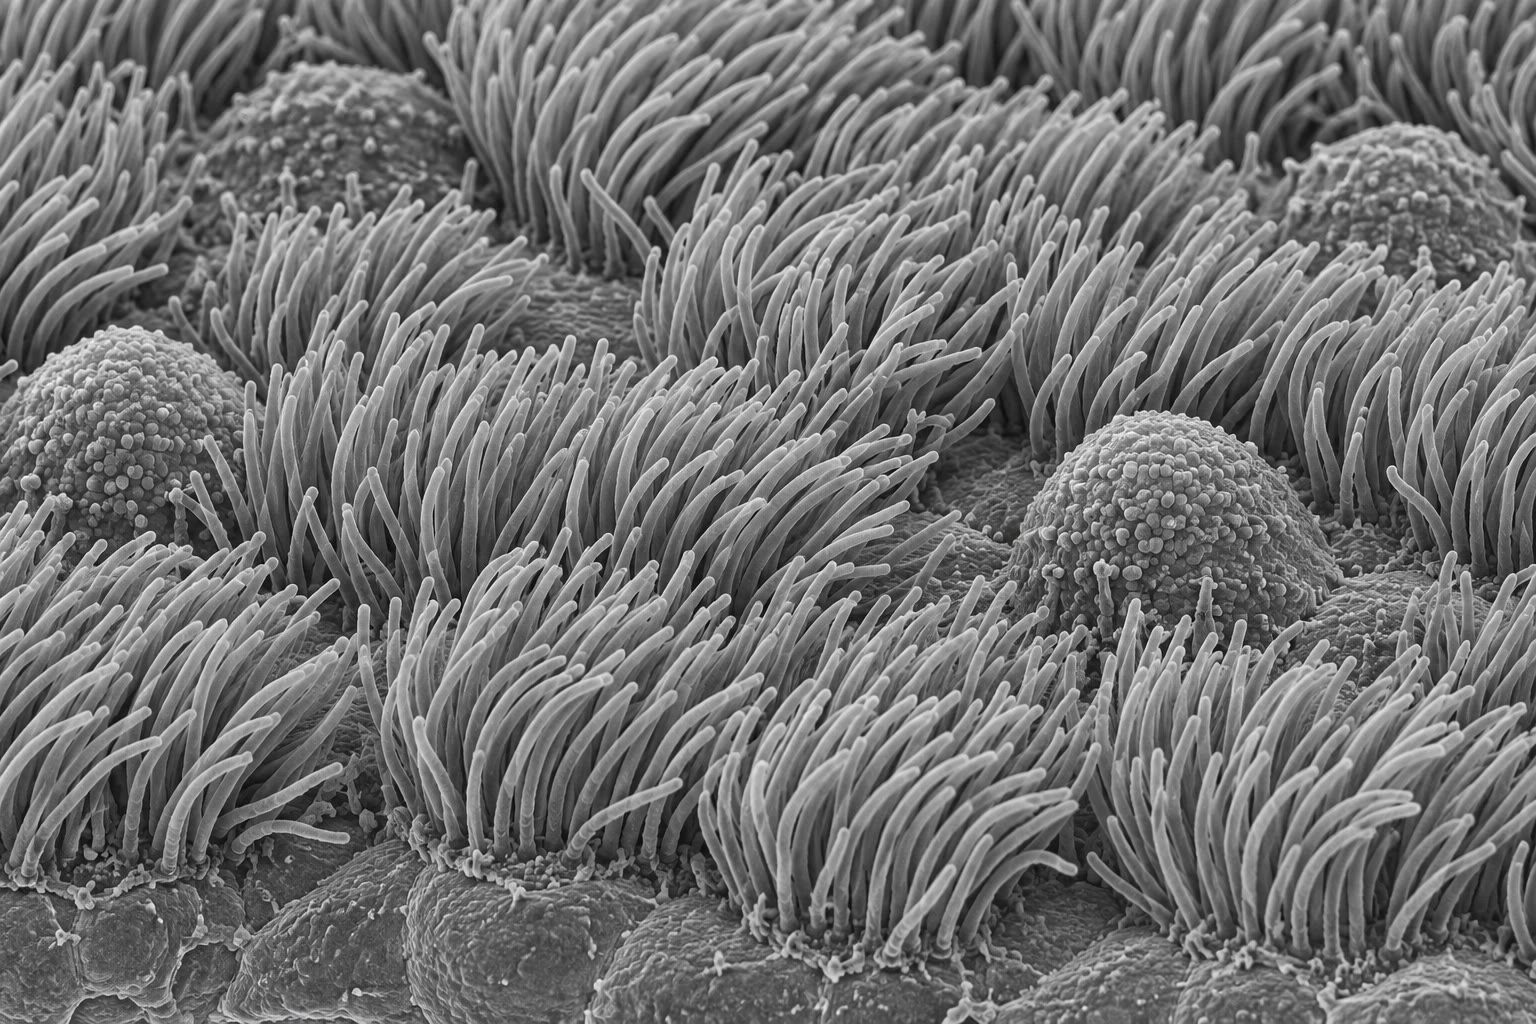
\includegraphics[width=0.54\linewidth]{images/book5/ai/b5-09-cilia-sem.jpg}\hspace{0.03\linewidth}
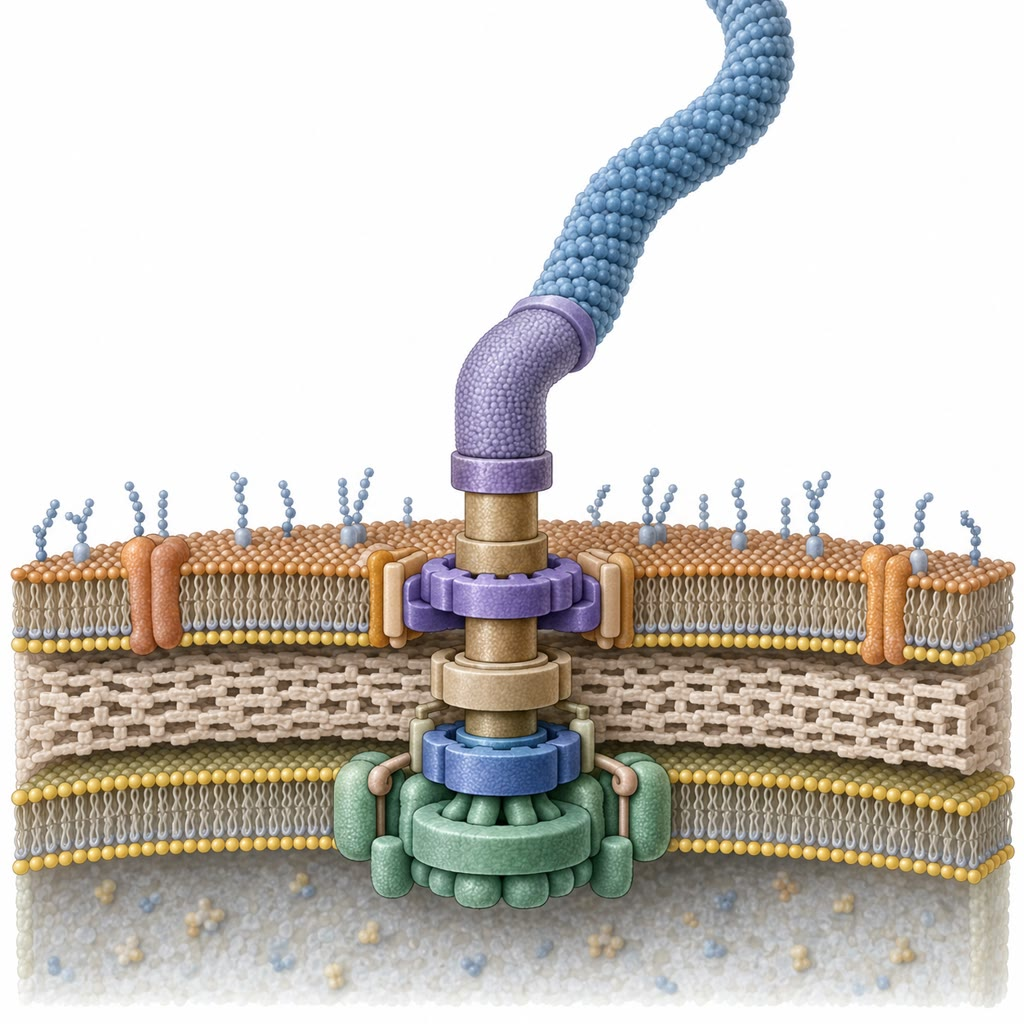
\includegraphics[width=0.36\linewidth]{images/book5/ai/b5-09-flagellar-motor.jpg}

{\small Links: het trilhaarepitheel van de luchtpijp in de
rasterelektronenmicroscoop, een grasveld van trilharen tussen
koepelvormige slijmproducerende cellen. Rechts: de \omterm{prop:b3:cytoskeleton-motility:flagellar-motor}{flagellaire motor}
van een bacterie, een draaimotor van ringen in het celomhulsel,
aangedreven door de stroom van protonen.}
\end{omfigure}

\begin{proposition}[De flagellaire motor van een bacterie]\label{prop:b3:cytoskeleton-motility:flagellar-motor}
\index{flagellaire motor}\index{rennen en tuimelen}
De zweepstaart van een bacterie is niet verwant aan die van een
eukaryoot: een stijf helicaal filament van flagelline, \qty{20}{nm} dik
en enkele micrometers lang, gedraaid door een \emph{draaimotor} die in
het celomhulsel is ingebed --- een rotor van zo'n vijfenveertig
eiwitten omringd door een ring van statoreenheden, elk een kanaal
waardoor protonen langs hun gradiënt de cel in stromen, ongeveer
duizend protonen per omwenteling. De motor draait tot \qty{300}{Hz},
keert binnen een milliseconde van richting om en ontwikkelt een koppel
van zo'n \qty{1000}{pN.nm}; hij is uit ongeveer twintig eiwitten
gebouwd waarvan de genen worden aangezet in de volgorde waarin de
onderdelen worden gemonteerd, van binnen naar buiten. Bij
\emph{E.~coli} bundelt de draaiing linksom de verscheidene
zweepstaarten tot een schroef en \emph{rent} de cel rechtdoor; een
omschakeling naar rechtsom blaast de bundel uiteen en \emph{tuimelt} de
cel naar een nieuwe willekeurige richting. De chemotaxisroute
beïnvloedt niets dan de frequentie van de tuimelingen --- minder zodra
de omstandigheden verbeteren --- en dat volstaat om een gradiënt op te
klimmen.
\end{proposition}

\begin{remark}[Het cytoskelet is een werkwoord]\label{rem:b3:cytoskeleton-motility:verb}
Vrijwel niets in dit hoofdstuk is een structuur in de zin waarin een
bot dat is: het \omterm{def:b3:cytoskeleton-motility:migration}{lamellipodium} is een golf van polymerisatie, de
spoelfiguur van \cref{ch:b3:cell-cycle-apoptosis} een
evenwichtstoestand van groeiende en instortende \omterm{def:b3:cytoskeleton-motility:filaments}{microtubuli}, de slag
van het \omterm{def:b3:cytoskeleton-motility:cilia}{trilhaar} een schakelpatroon van motoren. De omzet is geen prijs
die de cel erbij neemt maar het mechanisme zelf, en daarom draait elk
van deze systemen op de hydrolyse van nucleotiden en staat het binnen
minuten stil zodra het ATP opraakt, en daarom zijn de vergiften die de
polymeren in beide toestanden bevriezen --- taxol of colchicine,
falloïdine of cytochalasine --- even dodelijk.
\end{remark}

\section{Opgaven}

\begin{exercise}[$\star$]\label{exo:b3:cytoskeleton-motility:1}
Vergelijk \omterm{def:b3:cytoskeleton-motility:filaments}{actinefilamenten}, \omterm{def:b3:cytoskeleton-motility:filaments}{microtubuli} en \omterm{def:b3:cytoskeleton-motility:filaments}{intermediaire filamenten}
naar diameter, subeenheid, polariteit, nucleotide en gebruikelijke rol.
\end{exercise}

\begin{exercise}[$\star$]\label{exo:b3:cytoskeleton-motility:2}
Definieer de \omterm{thm:b3:cytoskeleton-motility:treadmilling}{kritische concentratie}. Waarom hebben de twee uiteinden
van een \omterm{def:b3:cytoskeleton-motility:filaments}{actinefilament} verschillende \omterm{thm:b3:cytoskeleton-motility:treadmilling}{kritische concentraties}, en wat
zou er gebeuren als zij gelijk waren?
\end{exercise}

\begin{exercise}[$\star$]\label{exo:b3:cytoskeleton-motility:3}
Noem voor elk een motor: een blaasje naar de celrand over \omterm{def:b3:cytoskeleton-motility:filaments}{microtubuli};
een blaasje naar het centrum; de samentrekking van een spanningsvezel;
het buigen van een \omterm{def:b3:cytoskeleton-motility:cilia}{trilhaar}. Geef de richting die elk op zijn baan
neemt.
\end{exercise}

\begin{exercise}[$\star$]\label{exo:b3:cytoskeleton-motility:4}
Noem de vier stappen van de kruipcyclus en het GTPase van de
Rho-familie dat elk van de eerste drie bestuurt.
\end{exercise}

\begin{exercise}[$\star\star$]\label{exo:b3:cytoskeleton-motility:5}
Het plusuiteinde van een polymeer heeft $k_{\text{on}} = \qty{5}{\micro M^{-1}.s^{-1}}$
en $k_{\text{off}} = \qty{1}{s^{-1}}$, het minuiteinde $k_{\text{on}} =
\qty{1}{\micro M^{-1}.s^{-1}}$ en $k_{\text{off}} = \qty{0.8}{s^{-1}}$.
Bepaal de twee \omterm{thm:b3:cytoskeleton-motility:treadmilling}{kritische concentraties}, de evenwichtsconcentratie en de
treadmillingsnelheid in subeenheden per seconde en, voor subeenheden van
\qty{2.7}{nm}, in nanometer per seconde.
\end{exercise}

\begin{exercise}[$\star\star$]\label{exo:b3:cytoskeleton-motility:6}
\omterm{def:b3:cytoskeleton-motility:motors}{Kinesine} loopt met \qty{800}{nm/s} in stappen van \qty{8}{nm}, elk één
ATP. Hoeveel ATP per seconde per motor? Het axon van een neuron is
\qty{1}{m}: hoe lang duurt de reis, en hoeveel ATP besteedt één motor
eraan? Vergelijk met de diffusietijd uit
\cref{prop:b3:cytoskeleton-motility:physics}.
\end{exercise}

\begin{exercise}[$\star\star$]\label{exo:b3:cytoskeleton-motility:7}
\omterm{def:b3:cytoskeleton-motility:motors}{Myosine} V zet per ATP een stap van \qty{36}{nm}. Wat is zijn maximale
\omterm{prop:b3:cytoskeleton-motility:physics}{blokkeerkracht}, en waarom is die lager dan die van \omterm{def:b3:cytoskeleton-motility:motors}{kinesine}? Welke
motor is geschikter voor een zware last, en welke om snel te bewegen?
\end{exercise}

\begin{exercise}[$\star\star$]\label{exo:b3:cytoskeleton-motility:8}
Voorspel het effect op een delende cel en op een kruipende cel van (a)
taxol, (b) colchicine, (c) cytochalasine, (d) een Rac-remmer, en
verklaar elk uit het mechanisme.
\end{exercise}

\begin{exercise}[$\star\star$]\label{exo:b3:cytoskeleton-motility:9}
In een FRAP-experiment op een \omterm{def:b3:cytoskeleton-motility:migration}{lamellipodium} keert de fluorescentie met
een halveringstijd van \qty{20}{s} terug tot \qty{90}{\%} van haar
beginwaarde. Wat zijn de verblijfstijd van actine in het netwerk en de
onbeweeglijke fractie? De spikkels stromen met \qty{1.5}{\micro m/min}
naar achteren terwijl de rand met \qty{1}{\micro m/min} vooruitgaat: met
welke snelheid polymeriseert het actine aan de rand?
\end{exercise}

\begin{exercise}[$\star\star\star$]\label{exo:b3:cytoskeleton-motility:10}
Verklaar de \omterm{def:b3:cytoskeleton-motility:instability}{dynamische instabiliteit} met de \omterm{def:b3:cytoskeleton-motility:instability}{GTP-kap}, en laat zien
waarom een populatie \omterm{def:b3:cytoskeleton-motility:filaments}{microtubuli} die net boven de \omterm{thm:b3:cytoskeleton-motility:treadmilling}{kritische
concentratie} wordt gehouden bimodaal wordt in lengte in plaats van
uniform. Wat wint de cel met een gedrag dat GTP verspilt?
\end{exercise}

\begin{exercise}[$\star\star\star$]\label{exo:b3:cytoskeleton-motility:11}
Een bacterie van \qty{2}{\micro m} zwemt met \qty{25}{\micro m/s}. In
water overheerst op deze schaal de viskeuze weerstand en staat de cel
binnen een nanometer stil zodra de motor stopt. Leg uit waarom een
heen-en-weergaande beweging (een roeispaan) haar niet kan voortstuwen en
een draaiende helix wel, en schat het aantal protonen dat de motor bij
\qty{100}{Hz} per seconde verbruikt.
\end{exercise}

\begin{exercise}[$\star\star\star$]\label{exo:b3:cytoskeleton-motility:12}
Het syndroom van Kartagener --- onbeweeglijke trilharen --- geeft
chronische bronchitis, mannelijke onvruchtbaarheid en bij de helft van
de patiënten een hart aan de rechterkant. Verklaar elk daarvan uit de
biologie van het \omterm{def:b3:cytoskeleton-motility:cilia}{axoneem}, en zeg waarom het laatste maar de helft
treft.
\end{exercise}

\section{Vraagstuk: een neutrofiel op pad}

\begin{problem}[{Weekendvraagstuk --- de actinebegroting van een
neutrofiel geteld, haar treadmilling berekend, de reis van een blaasje
door een axon tegen de diffusie afgezet, het rendement van een motor
gemeten, en de polymerisatie en de ATP-kosten van het kruipende front
uitgewerkt, met als besluit de treadmillingsnelheid, de tijd om een
axon over te steken en de ATP die een lamellipodium per seconde
verstookt}]
\label{pb:b3:cytoskeleton-motility:1}
Gegevens: een neutrofiel met een volume van \qty{300}{\micro m^3}
bevat actine op \qty{200}{\micro M}, half gepolymeriseerd; een
subeenheid voegt \qty{2.7}{nm} aan een filament toe. Snelheidsconstanten
van actine als in
\cref{ex:b3:cytoskeleton-motility:actin-numbers}. \omterm{def:b3:cytoskeleton-motility:motors}{Kinesine}: stappen van
\qty{8}{nm}, \qty{800}{nm/s}, \omterm{prop:b3:cytoskeleton-motility:physics}{blokkeerkracht} \qty{6}{pN}; ATP-hydrolyse
$\Delta G = \qty{50}{kJ/mol}$; $k_{B}T = \qty{4.1}{pN.nm}$;
diffusiecoëfficiënt van een blaasje \qty{1}{\micro m^2/s}; axonlengte
\qty{1}{m}. Het \omterm{def:b3:cytoskeleton-motility:migration}{lamellipodium} is \qty{20}{\micro m} breed met $200$
filamenten per micrometer rand, en gaat \qty{10}{\micro m/min} vooruit;
het netwerk valt \qty{3}{\micro m} achter de rand uiteen.

\medskip
\noindent\textbf{Deel I --- De actinebegroting.}
\begin{enumerate}
  \item Hoeveel actinemoleculen bevat de cel, en hoeveel zitten er in
        filamenten?
  \item Welke totale filamentlengte is dat? Hoeveel filamenten zijn
        het, als een filament gemiddeld \qty{0.25}{\micro m} is?
  \item Het vrije actine is \qty{100}{\micro M}, ver boven de \omterm{thm:b3:cytoskeleton-motility:treadmilling}{kritische
        concentratie} van het gekartelde uiteinde. Waarom groeien de
        filamenten niet eenvoudig tot het monomeer op is? (Twee
        eiwitten.)
  \item Treadmilling in vitro: bereken $C_{\text{ss}}$ en $J$ uit de
        snelheidsconstanten, en de treadmillingsnelheid in nanometer per
        seconde en in micrometer per minuut.
  \item In de cel is de werkelijke snelheid \qty{1}{\micro m/min}. Met
        welke factor versnellen de regulatoren het kale polymeer?
  \item Elke subeenheid die door het filament trekt kost één ATP. Als
        alle $2\times 10^{5}$ filamenten met de celsnelheid aan
        treadmilling deden, hoeveel ATP per seconde is dat, en welk deel
        is dat van de totale omzet van een cel van ongeveer $10^{9}$ ATP
        per seconde?
\end{enumerate}

\medskip
\noindent\textbf{Deel II --- Een blaasje door het axon.}
\begin{enumerate}[resume]
  \item Hoe lang doet een blaasje dat door \omterm{def:b3:cytoskeleton-motility:motors}{kinesine} wordt getrokken over
        het axon, en hoeveel stappen en ATP besteedt de motor eraan?
  \item Hoe lang zou de diffusie over \qty{1}{m} duren? En over
        \qty{10}{\micro m}, de breedte van een cellichaam? Wat zegt de
        vergelijking over waar cellen zich op diffusie kunnen verlaten?
  \item Bereken de energie per ATP in joule en in eenheden $k_{B}T$.
  \item Bereken de maximale kracht van een motor met stappen van
        \qty{8}{nm}, en het rendement van \omterm{def:b3:cytoskeleton-motility:motors}{kinesine} bij blokkering.
  \item Een blaasje met straal \qty{100}{nm} in cytoplasma met
        viscositeit \qty{0.01}{Pa.s} (tien keer water) dat met
        \qty{800}{nm/s} beweegt ondervindt een weerstand
        $F = 6\pi\eta r v$. Bereken die, en vergelijk met de
        \omterm{prop:b3:cytoskeleton-motility:physics}{blokkeerkracht}: hoeveel motoren zijn er nodig?
  \item Het axon van een neuron draagt ongeveer $10^{4}$ blaasjes
        tegelijk. Wat is het totale ATP-verbruik van het transport per
        seconde, en hoe verhoudt dat zich tot de kosten van het vuren
        van het neuron, ongeveer $10^{9}$ ATP per seconde? Wat betekent
        dit voor een neuron waarin de mitochondriën het laten afweten?
\end{enumerate}

\medskip
\noindent\textbf{Deel III --- Het front.}
\begin{enumerate}[resume]
  \item Reken de randsnelheid om naar nanometer per seconde, en bereken
        hoeveel subeenheden per seconde elk filament moet toevoegen om
        bij te blijven.
  \item Hoeveel filamenten duwen tegen de rand, en hoeveel subeenheden
        per seconde verbruikt de hele rand?
  \item Elke toegevoegde subeenheid is één gehydrolyseerd ATP dat later
        wordt hergebruikt. Bereken de ATP per seconde voor de
        uitstulping en het deel van de $10^{9}$ per seconde van de cel.
  \item Het netwerk achter de rand is \qty{3}{\micro m} diep en valt
        daar uiteen. Wat is de levensduur van een subeenheid in het
        netwerk, en hoeveel subeenheden zitten er op elk moment in?
  \item Het membraan biedt weerstand aan de uitstulping met een kracht
        van ongeveer \qty{1}{pN} per filament. Bereken de arbeid per
        toegevoegde subeenheid ($F\times \qty{2.7}{nm}$) in $k_{B}T$ en
        zeg of de brownse ratel --- een thermische schommeling die een
        spleet van \qty{2.7}{nm} opent --- aannemelijk is.
  \item Waarom heeft de komeetstaart van Listeria geen motor
        nodig, en hoe hard kan zij duwen als zij dezelfde machinerie
        aantrekt?
\end{enumerate}

\medskip
\noindent\textbf{Deel IV --- Richting.}
\begin{enumerate}[resume]
  \item De neutrofiel neemt een lokstof waar waarvan de concentratie
        over haar breedte van \qty{10}{\micro m} met \qty{2}{\%} stijgt.
        Hoeveel meer receptoren zijn er met \num{50000} receptoren en
        een $K_{d}$ gelijk aan de gemiddelde concentratie bezet op de
        voorste helft dan op de achterste? (Bezetting $\theta = C/(C +
        K_{d})$; neem per kant de helft van de receptoren.)
  \item De toevallige schommeling in het aantal bezette receptoren aan
        één kant is ongeveer de wortel uit dat aantal. Is het verschil
        uit vraag 19 op één enkel moment waarneembaar? Hoe helpt
        middelen over enkele seconden?
  \item Welk GTPase moet vooraan en welk achteraan worden geactiveerd
        opdat de cel zich naar de bron draait? Wat zou een cel doen die
        overal constitutief actief Rac heeft?
  \item De cel bereikt de bacterie in \qty{3}{min} vanaf
        \qty{30}{\micro m} afstand. Toets de snelheid aan de gegevens.
  \item Een cel zonder Arp2/3 beweegt in plaats daarvan met blebbing
        --- door druk gedreven uitstulpingen van membraan. Welke stap
        van de cyclus is vervangen, en wat zegt dat over de rol van
        actine in de overige stappen?
  \item De hele kruipcyclus duurt minuten, en toch draait de cel binnen
        seconden wanneer de gradiënt verschuift. Verklaar dat met de
        levensduur van het netwerk uit vraag~16.
  \item Vat samen: de treadmillingsnelheid in vitro (vraag~4), de tijd
        die een blaasje over het axon doet (vraag~7), en de ATP per
        seconde die aan de uitstulping wordt besteed (vraag~15).
\end{enumerate}
\end{problem}
